\documentclass[t, final, 12pt, xcolor={usenames,dvipsnames}, table]{beamer}

\usepackage{xcolor}
\usepackage{listings}
%\usepackage{lstlinebgrd}
\usepackage[normalem]{ulem}
\useunder{\uline}{\ul}{}


 
\definecolor{codegreen}{rgb}{0,0.6,0}
\definecolor{codegray}{rgb}{0.5,0.5,0.5}
\definecolor{codepurple}{rgb}{0.58,0,0.82}
\definecolor{backcolour}{rgb}{0.95,0.95,0.92}

\lstset{
    basicstyle=\scriptsize\ttfamily,
    keywordstyle=\color{blue},
    identifierstyle=\color{black},
    commentstyle=\color{orange},
	stringstyle=\color{codepurple},
    showstringspaces=false,
    numberstyle=\color{gray}\tiny,
    breakatwhitespace=false,         
    breaklines=true,                 
    captionpos=b,                    
    keepspaces=true,                 
    numbers=left,                    
    numbersep=5pt,                  
    showspaces=false,                
    showstringspaces=false,
    showtabs=false,                  
    tabsize=2,
    extendedchars=\true,
    inputencoding=utf8,
    frame=tb, 
    columns=fixed,
    backgroundcolor=\color{red!32!green!33!blue!5},
    language=Python
}

\usetheme[pageofpages=of,
          alternativetitlepage=true,
          titlepagelogo=python-logo-big,
          ]{Torino}
          
\usecolortheme{freewilly}


\author{Luiz Alberto}
\title{Python para Ciência de Dados}
\subtitle{NumPy, Matplotlib, Pandas Introdutório}
\institute{Ciência da Computação}
\date{\today}

\logo{
\includegraphics[height=0.125\paperheight]{python-logo-small}}

\begin{document}
  
  \begin{frame}[t,plain]
    \titlepage
  \end{frame}
  
  % NumPy
  \begin{frame}[t, fragile]{NumPy}
  \begin{block}{\alert{Num}eric \alert{Py}thon:}
    Biblioteca para computação científica. Implementa arrays muldimensionais e permite a fácil execução de operações matemáticas  (\url{www.numpy.org}).
  \end{block}
  \begin{itemize}
    \item Utilizada em cálculos de alta performance de vetores e matrizes 
    \item Fornece versões pré-compiladas de funções numéricas
    \item Alternativa à Lista em Python: NumPy Array
    \item Cálculos sobre matrizes inteiras (broacasting)
    \item Escrita em C e Fortran
  \end{itemize}
\end{frame}
%
\begin{frame}[t, fragile]{NumPy}
  \lstinputlisting[language=python]{aula-2/codigos/numpy/numpy-basic-1.py}  
\end{frame}
%
\begin{frame}[t, fragile]{Comparação com listas}
  \lstinputlisting[language=python]{aula-2/codigos/numpy/numpy-basic-2.py}  
\end{frame}
%
\begin{frame}[t, fragile]{Subsetting}
  \lstinputlisting[language=python]{aula-2/codigos/numpy/numpy-basic-3.py}  
\end{frame}
%
\begin{frame}[t, fragile]{Arrays multidimensionais}
  \lstinputlisting[language=python]{aula-2/codigos/numpy/numpy-basic-4.py}  
\end{frame}
%
\begin{frame}[t, fragile, allowframebreaks]{Fatiamento}
  \lstinputlisting[language=python]{aula-2/codigos/numpy/numpy-basic-6.py}  
\end{frame}
%
\begin{frame}[t, fragile]{Estatística básica}
  \lstinputlisting[language=python]{aula-2/codigos/numpy/numpy-basic-7.py}  
\end{frame}
%
\begin{frame}[t, fragile]{Geração de dados}
  \lstinputlisting[language=python]{aula-2/codigos/numpy/numpy-basic-8.py}  
\end{frame}
%

 
 
  \begin{frame}[t, fragile]{Hora de colocar a mão na massa}
  \begin{enumerate}
  \item Salve na sua máquina o notebook \verb!numpy-maos-na-massa-1.ipynb! que está no endereço \url{https://github.com/gomesluiz/python-para-ciencia-de-dados/tree/master/notebooks}
  \item Abra o notebook no Jupyter do Anaconda e faça os exercícios.
  \end{enumerate}
\end{frame}

  % Pandas 
  \begin{frame}[t, fragile]{Pandas}
  \begin{block}{Definição:}
    Biblioteca para análise de dados. Fornece ferramentas para manipulação de estruturas de dados, como matrizes, vetores e dataframes(\url{www.pandas.pydata.org}). 
  \end{block}
  \begin{itemize}
    \item Pandas é uma biblioteca open-source com licença BSD
    \item Fornece ferramentas de alta performance e fáceis de utilizar para manipulação de estrutura de dados
    \item Escrita em Python
  \end{itemize}
\end{frame}
%
%
\begin{frame}[t, fragile]{Pandas}
  \begin{block}{Datasets:}
    Biblioteca para análise de dados. Fornece ferramentas para manipulação de estruturas de dados, como matrizes, vetores e dataframes(\url{www.pandas.pydata.org}). 
  \end{block}
  \begin{itemize}
    \item Pandas é uma biblioteca open-source com licença BSD
    \item Fornece ferramentas de alta performance e fáceis de utilizar para manipulação de estrutura de dados
    \item Escrita em Python
  \end{itemize}
\end{frame}
%
 
 
  \begin{frame}[t, fragile]{Pandas Series}
  \begin{block}{Definição}
    Objeto que representa uma estrutura de dados unidimensional similar ao array mas com algumas características a mais.
  \end{block}
  \begin{columns}
    \begin{column}{0.5\textwidth}
        \begin{itemize}
          \item Composta por dois arrays:
          \item (i) dados
          \item (ii) índice
        \end{itemize}
    \end{column}

    \begin{column}{0.5\textwidth}
      \begin{center}
        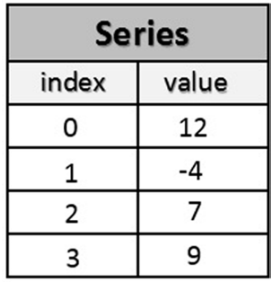
\includegraphics[scale=.40]{aula-2/figuras/pandas-series-1.png}
      \end{center}
    \end{column}
  \end{columns}
\end{frame}
%
\begin{frame}[t, fragile, allowframebreaks]{Declarando uma Serie}
  \begin{itemize}
    \item Índice padrão
  \end{itemize}
  \lstinputlisting[language=python]{aula-2/codigos/pandas/pandas-series-1.py}  
  \framebreak
  \begin{itemize}
    \item Índice personalizado
  \end{itemize}
  Livro: O Perfil das Empresas Brasilieiras em Gestão e Governança de Dados
  \lstinputlisting[language=python]{aula-2/codigos/pandas/pandas-series-2.py}  
\end{frame}
\begin{frame}[t, fragile]{Acessando índices e valores}
  \lstinputlisting[language=python]{aula-2/codigos/pandas/pandas-series-3.py}  
\end{frame}
%
\begin{frame}[t, fragile]{Selecionando valores em uma Serie}
  \lstinputlisting[language=python]{aula-2/codigos/pandas/pandas-series-4.py}  
\end{frame}
%
\begin{frame}[t, fragile]{Atribuindo valores}
  \lstinputlisting[language=python]{aula-2/codigos/pandas/pandas-series-5.py}  
\end{frame}
%
\begin{frame}[t, fragile]{Filtrando valores}
  \lstinputlisting[language=python]{aula-2/codigos/pandas/pandas-series-6.py}  
\end{frame}
%
\begin{frame}[t, fragile, allowframebreaks]{Avaliando valores}
  \lstinputlisting[language=python]{aula-2/codigos/pandas/pandas-series-7.py}  
\end{frame}
%

  \begin{frame}[t, fragile]{Pandas Dataframes}
  \begin{block}{Definição}
    Estrutura de dados tabular muito similar a uma planilha..
  \end{block}
  \begin{columns}
    \begin{column}{0.5\textwidth}
        \begin{itemize}
          \item Estende a {\bf Serie} para multiplas dimensões
          \item Consiste de uma coleção ordenada de colunas
          \item Contém diversos valores com tipos diferentes
        \end{itemize}
    \end{column}

    \begin{column}{0.5\textwidth}
      \begin{center}
        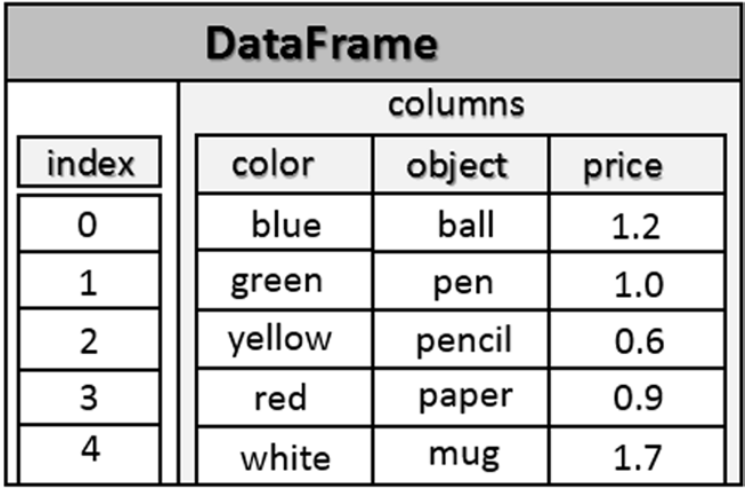
\includegraphics[scale=.21]{aula-2/figuras/pandas-dataframes-1.png}
      \end{center}
    \end{column}
  \end{columns}
\end{frame}
%
\begin{frame}[t, fragile, allowframebreaks]{Dataframe baseado em dicionário}
  \lstinputlisting[language=python]{aula-2/codigos/pandas/pandas-dataframes-1.py}  
\end{frame}
%
\begin{frame}[t, fragile, allowframebreaks]{Dataframe baseado em arquivo CSV}
  \lstinputlisting[language=python]{aula-2/codigos/pandas/pandas-dataframes-2.py}  
\end{frame}
%
\begin{frame}[t, fragile, allowframebreaks]{Acesso a valores de colunas}
  \lstinputlisting[language=python, firstline=5]{aula-2/codigos/pandas/pandas-dataframes-3.py}  
\end{frame}
%
\begin{frame}[t, fragile]{Acesso a valores de linhas}
  \lstinputlisting[language=python, firstline=6]{aula-2/codigos/pandas/pandas-dataframes-4.py}  
\end{frame}
%
\begin{frame}[t, fragile]{Operador $[ ]$}
  \begin{itemize}
    \item \verb![ ]!: tem funcionalidade limitada 
    \item Idealmente:
    \begin{itemize}
      \item para arrays bidimensionais
      \item \verb!um_array[linha, coluna]!
    \end{itemize}
    \item Em Pandas:
    \begin{itemize}
      \item \verb!loc!  (baseado em conteúdo)
      \item \verb!iloc! (baseado em posição)
    \end{itemize}
  \end{itemize}
\end{frame}
%
\begin{frame}[t, fragile]{Acesso a valores de linhas com {\bf loc}}
  \lstinputlisting[language=python, firstline=6]{aula-2/codigos/pandas/pandas-dataframes-5.py}  
\end{frame}
%
\begin{frame}[t, fragile]{Acesso a valores de linhas e colunas com {\bf loc}}
  \lstinputlisting[language=python, firstline=6]{aula-2/codigos/pandas/pandas-dataframes-6.py}  
\end{frame}
%
\begin{frame}[t, fragile]{Recapitulando}
  \begin{itemize}
    \item Colchetes \verb![ ]! 
    \begin{itemize}
      \item acesso a colunas: \verb!brics[["pais", "capital"]]!  
      \item acesso a linhas: somente via fatiamento \verb!brics[1:4]!
    \end{itemize}
    \item {\bf loc}
    \begin{itemize}
      \item acesso a linhas: \verb!brics.loc[["RU", "IN", "CH"]]!  
      \item acesso a colunas: \verb!brics.loc[:, ["pais", "capital"]]! 
      \item linhas e colunas: \verb!brics.loc[["RU", "IN", "CH"], ["pais", "capital"]]!    
    \end{itemize}
  \end{itemize}
\end{frame}
%
\begin{frame}[t, fragile]{Acesso a valores de linhas com {\bf iloc}}
  \lstinputlisting[language=python, firstline=6]{aula-2/codigos/pandas/pandas-dataframes-7.py}  
\end{frame}
%

\begin{frame}[t, fragile]{Acesso a valores de linhas e colunas com {\bf iloc}}
  \lstinputlisting[language=python, firstline=6]{aula-2/codigos/pandas/pandas-dataframes-8.py}  
\end{frame}
%



  \begin{frame}[t, fragile, allowframebreaks]{Hora de colocar a mão na massa}
  Salvar cada um dos exercícios a seguir em um arquivo separado.
\end{frame}
  
   % Matplotlib
  \begin{frame}[t, fragile]{Matplotlib}
  \begin{block}{Definição:}
    Biblioteca python para plotagem de gráficos 2D (incluindo 3D)   (\url{www.matplotlib.org}). 
  \end{block}
  \begin{itemize}
    \item Simplicidade de utilização
    \item Desenvolvimento gradual e interativo
    \item Grande controle sobre os elementos gráficos
    \item Exportação em formatos PNG, PDF, SVG e EPS 
  \end{itemize}
\end{frame}
%
\begin{frame}[t, fragile]{Vizualização de Dados}
  \begin{itemize}
    \item Muito importante na visualização de dados
    \begin{itemize}
      \item Explorar os dados
      \item Apresentar "insights"
    \end{itemize}
  \end{itemize}
  \begin{figure}
    
\includegraphics[scale=.30]{aula-2/figuras/matplot-dataviz-a.jpg}
  \end{figure}
\end{frame}
%

 
  \begin{frame}[t, fragile]{Line plot}
  \begin{columns}
    \begin{column}{0.5\textwidth}
        \lstinputlisting[language=python]{aula-2/codigos/matplotlib/matplotlib-lineplot-1.py}  
    \end{column}

    \begin{column}{0.5\textwidth}
      \begin{center}
        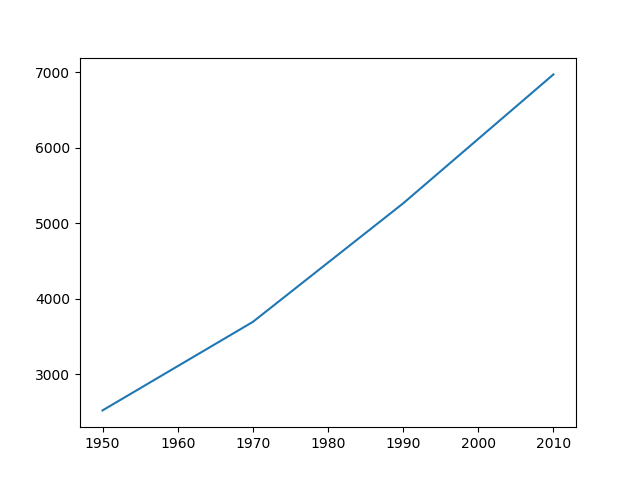
\includegraphics[scale=.40]{aula-2/figuras/matplotlib-lineplot-1.png}
      \end{center}
    \end{column}
  \end{columns}
\end{frame}
%

 
  \begin{frame}[t, fragile]{Scatter plot}
  \begin{columns}
    \begin{column}{0.5\textwidth}
        \lstinputlisting[language=python]{aula-2/codigos/matplotlib/matplotlib-scatterplot-1.py}  
    \end{column}

    \begin{column}{0.5\textwidth}
      \begin{center}
        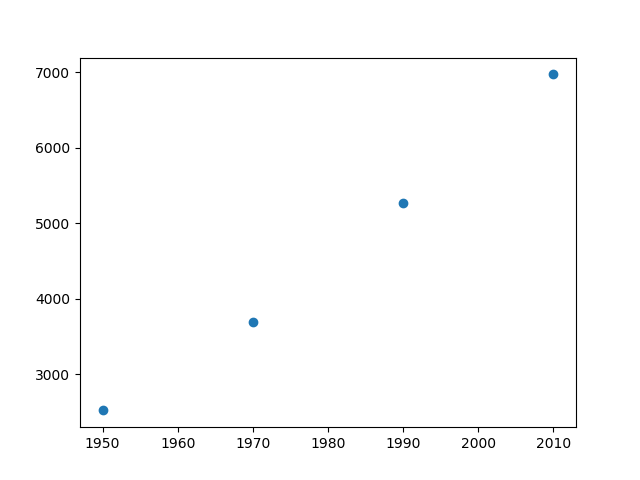
\includegraphics[scale=.40]{aula-2/figuras/matplotlib-scatterplot-1.png}
      \end{center}
    \end{column}
  \end{columns}
\end{frame}
%

 
  \begin{frame}[t, fragile]{Histogram}
  \begin{itemize}
    \item Utilizado para explorar dados
    \item Fornece uma idea da distribuição dos dados
  \end{itemize}
  \begin{figure}
    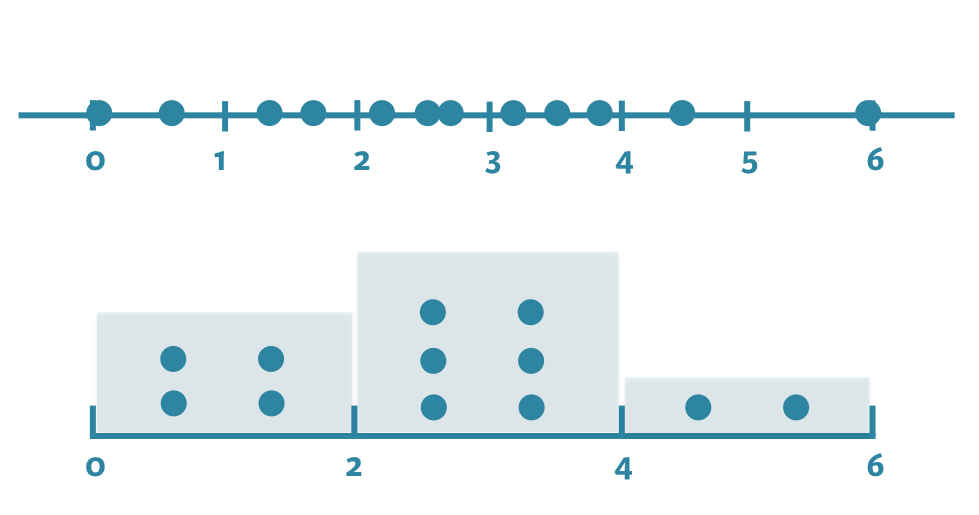
\includegraphics[scale=.40]{aula-2/figuras/matplotlib-histogram-a.png}
  \end{figure}

\end{frame}
%
\begin{frame}[t, fragile]{Histogram}
  \begin{columns}
    \begin{column}{0.5\textwidth}
        \lstinputlisting[language=python]{aula-2/codigos/matplotlib/matplotlib-histogram-1.py}  
    \end{column}

    \begin{column}{0.5\textwidth}
      \begin{center}
        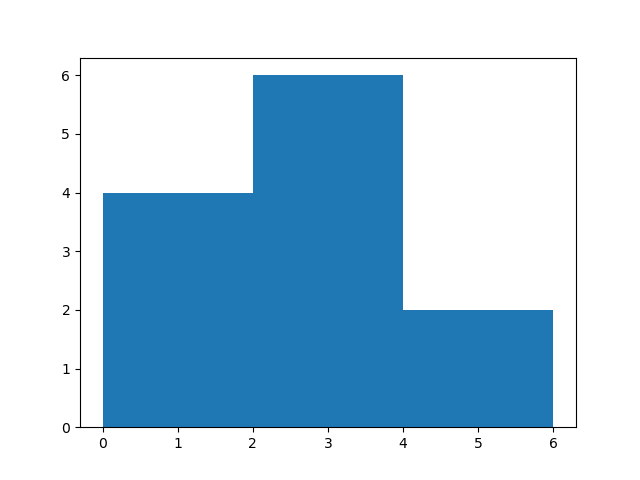
\includegraphics[scale=.40]{aula-2/figuras/matplotlib-histogram-1.png}
      \end{center}
    \end{column}
  \end{columns}
\end{frame}
%

 
  \begin{frame}[t, fragile]{Customização}
  \begin{itemize}
    \item Existem muitas opções
    \begin{itemize}
      \item Diferentes tipos de gráficos
      \item Diversas customizações
    \end{itemize}
    \item A escolha depende
    \begin{itemize}
      \item Dados
      \item Estória a ser contada
    \end{itemize}
  \end{itemize}
\end{frame}
%
\begin{frame}[t, fragile]{Customização}
  \begin{columns}
    \begin{column}{0.55\textwidth}
        \lstinputlisting[language=python]{aula-2/codigos/matplotlib/matplotlib-customization-1.py}  
    \end{column}

    \begin{column}{0.45\textwidth}
      \begin{center}
        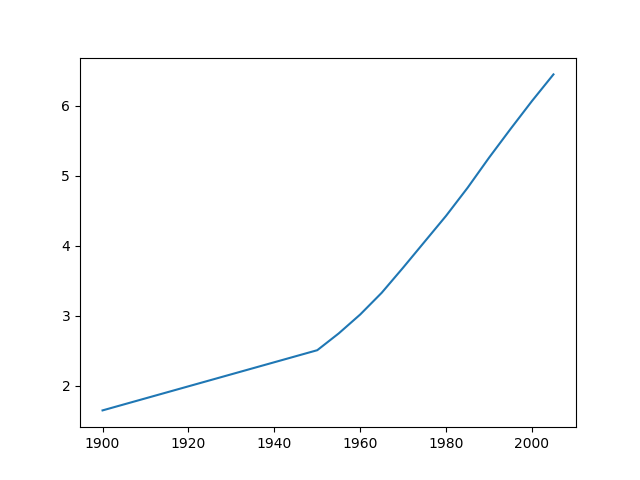
\includegraphics[scale=.35]{aula-2/figuras/matplotlib-customization-1.png}
      \end{center}
    \end{column}
  \end{columns}
\end{frame}
%
\begin{frame}[t, fragile]{Títulos dos eixos X e Y}
  \begin{columns}
    \begin{column}{0.55\textwidth}
        \lstinputlisting[language=python]{aula-2/codigos/matplotlib/matplotlib-customization-2.py}  
    \end{column}

    \begin{column}{0.45\textwidth}
      \begin{center}
        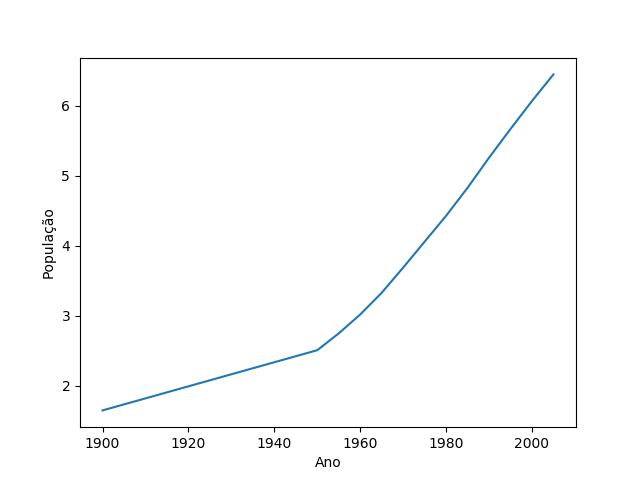
\includegraphics[scale=.35]{aula-2/figuras/matplotlib-customization-2.png}
      \end{center}
    \end{column}
  \end{columns}
\end{frame}
%
\begin{frame}[t, fragile]{Título Principal}
  \begin{columns}
    \begin{column}{0.55\textwidth}
        \lstinputlisting[language=python, firstline=12]{aula-2/codigos/matplotlib/matplotlib-customization-3.py}  
    \end{column}

    \begin{column}{0.45\textwidth}
      \begin{center}
        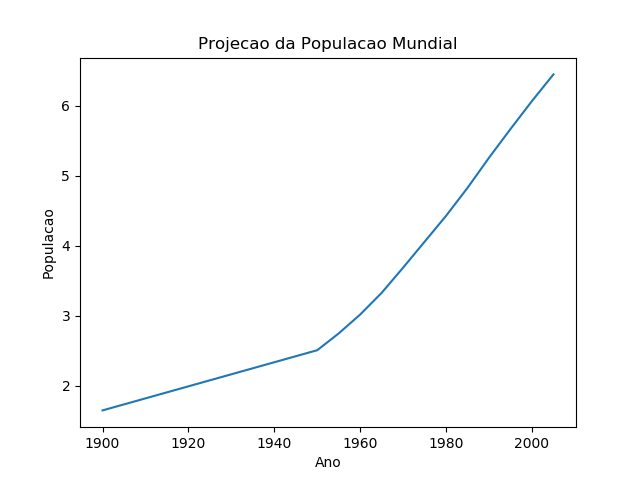
\includegraphics[scale=.35]{aula-2/figuras/matplotlib-customization-3.png}
      \end{center}
    \end{column}
  \end{columns}
\end{frame}
%
\begin{frame}[t, fragile, allowframebreaks]{Ticks}
  \begin{columns}
    \begin{column}{0.55\textwidth}
        \lstinputlisting[language=python, firstline=12]{aula-2/codigos/matplotlib/matplotlib-customization-4.py}  
    \end{column}

    \begin{column}{0.45\textwidth}
      \begin{center}
        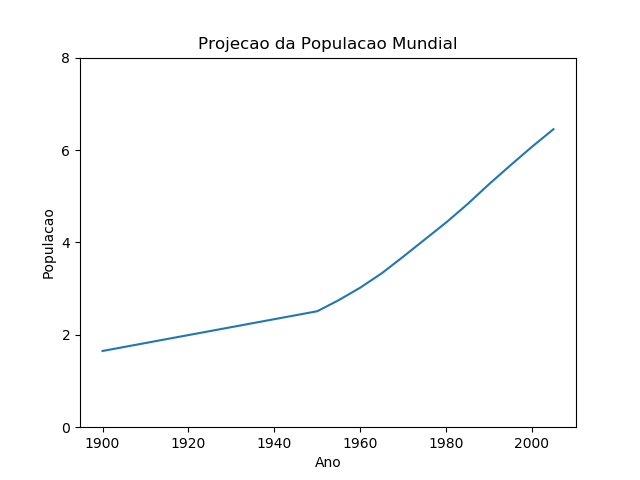
\includegraphics[scale=.35]{aula-2/figuras/matplotlib-customization-4.png}
      \end{center}
    \end{column}
  \end{columns}
  
  \framebreak
  
  \begin{columns}
    \begin{column}{0.55\textwidth}
        \lstinputlisting[language=python, firstline=12]{aula-2/codigos/matplotlib/matplotlib-customization-5.py}  
    \end{column}

    \begin{column}{0.45\textwidth}
      \begin{center}
        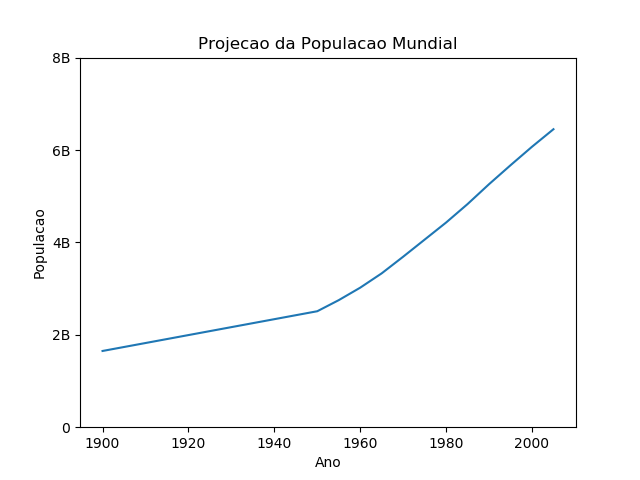
\includegraphics[scale=.35]{aula-2/figuras/matplotlib-customization-5.png}
      \end{center}
    \end{column}
  \end{columns}
\end{frame}
%
\begin{frame}[t, fragile]{Adicionando Dados Históricos}
  \begin{columns}
    \begin{column}{0.55\textwidth}
        \lstinputlisting[language=python, firstline=12]{aula-2/codigos/matplotlib/matplotlib-customization-6.py}  
    \end{column}

    \begin{column}{0.45\textwidth}
      \begin{center}
        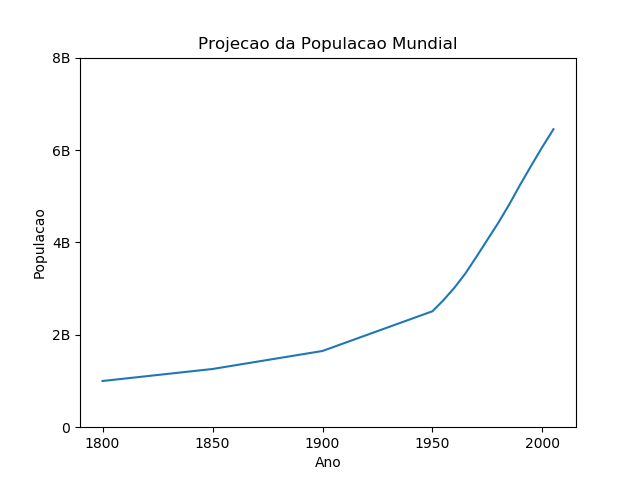
\includegraphics[scale=.35]{aula-2/figuras/matplotlib-customization-6.png}
      \end{center}
    \end{column}
  \end{columns} 
\end{frame}
%
%
\begin{frame}[t, fragile]{Antes x Depois}
  \begin{columns}
    \begin{column}{0.5\textwidth}
      \begin{figure}
        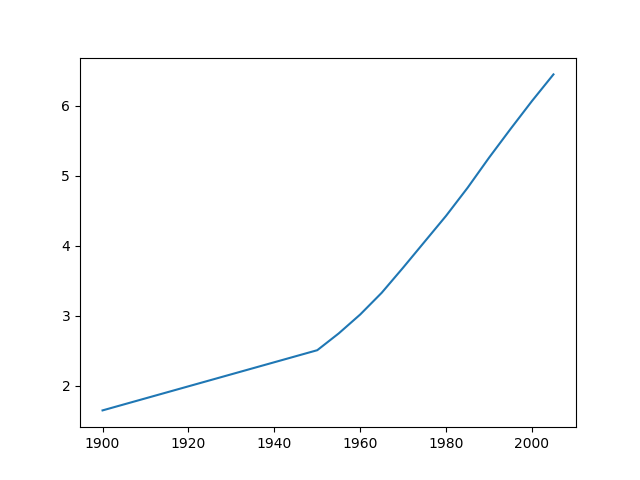
\includegraphics[scale=.35]{aula-2/figuras/matplotlib-customization-1.png}
      \end{figure}
    \end{column}

    \begin{column}{0.5\textwidth}
      \begin{figure}
        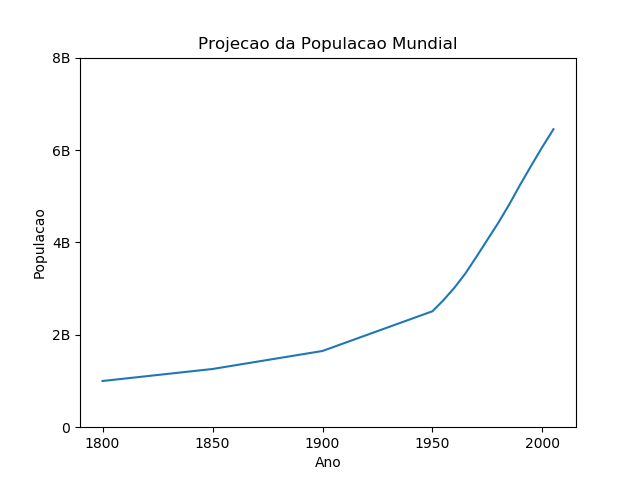
\includegraphics[scale=.35]{aula-2/figuras/matplotlib-customization-6.png}
      \end{figure}
    \end{column}
  \end{columns} 
\end{frame}


  \begin{frame}[t, fragile, allowframebreaks]{Hora de colocar a mão na massa}
  Salvar cada um dos exercícios a seguir em um arquivo separado.
\end{frame}


  
\end{document}

